\chapter{Introduzione teorica}\label{chap:introduzione_teorica}
Nel seguente capitolo verranno introdotte le basi teoriche utili alla comprensione del presente lavoro.
In particolare vedremo prima gli alberi di sintassi astratta, utilizzati per la generazione del modello, e poi sommariamente il modello Code2Vec, introdotto per la prima volta nella ricerca \cite{alon2019code2vec}, posto alla base del modello utilizzato che verrà discusso nel \autoref{chap:modello}.
Fondamenti di \ML{} e \DL{} non saranno invece trattati. 

\section{Albero di sintassi astratta}
Un albero di sintassi astratta, in breve \textit{ast} (dall'inglese \textit{abstract syntax tree}), è una rappresentazione ad albero della struttura sintattica astratta di un testo, nel nostro caso del codice sorgente.
Queste strutture sono spesso generate da parser specifici e vengono utilizzate come rappresentazione intermedia del programma in un processo di compilazione.
In maniera più formale, un albero di sintassi astratta per un frammento di codice $C$ è una tupla del tipo:
    \[(N, T, X, s, \delta, \phi)\]
dove $N$ è l'insieme dei nodi non terminali, $T$ l'insieme dei nodi terminali, $X$ un insieme di valori, s la radice,  $\delta$ la funzione che associa ad'un non terminale la lista di nodi figli e $\phi$ la funzione che associa ad'un terminale un valore.

Possiamo vedere un esempio di albero prendendo il frammento di codice nello \autoref{code:esempio} scritto in uno pseudo-linguaggio.
Un possibile albero di sintassi astratta per questo frammento di codice è quello indicato in \autoref{fig:ast_esempio}.
Come si può vedere l'\textit{ast} rappresenta in modo efficace la struttura completa del codice, andando ad individuare e distinguere elementi come:
  \begin{itemize}
    \item Il corpo, la \textit{signature} e il valore di ritorno della funzione. 
    \item La dichiarazione della variabile 'total' e il blocco del \textit{for}.
    \item I componenti del costrutto \textit{for}: il corpo, la condizione, l'inizializzazione e lo step della variabile di controllo.
  \end{itemize}

  \begin{code}[caption={Frammento di codice che calcola la somma dei valori in un vettore}, label={code:esempio}]
    void foo(int[] array){
      int totale = 0;
      for(int i = 0; i < array.length; i++){
        totale = totale + array[i]
      }
      return totale;
    }
  \end{code}
  \begin{figure}[h]
    \centering
    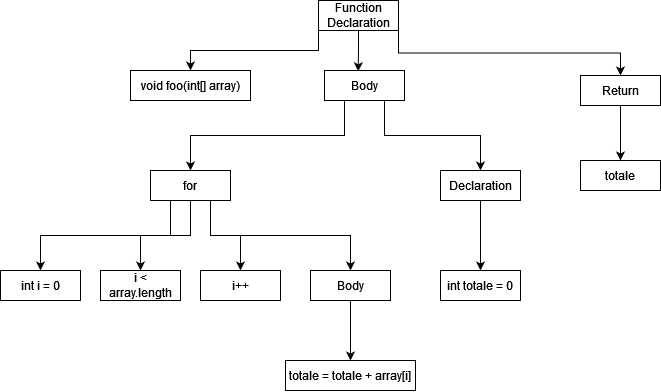
\includegraphics[scale=0.5]{images/astEsempio.png}
    \caption{Esempio di albero di sintassi astratta}
    \label{fig:ast_esempio}
  \end{figure}


\section{Code2Vec}\label{sec:code2vec}
Il modello Code2Vec, sviluppato nella ricerca \cite{alon2019code2vec}, ha come obbiettivo la rappresentazione di un \textit{code snippet}, di lunghezza variabile, come un vettore di lunghezza fissa.
Questa operazione di trasformazione viene detta \textit{embedding}.
Una volta effettuata questa trasformazione il vettore può essere poi utilizzato per ulteriori task come la predizione del nome del metodo, come studiato nel articolo, o, come nel caso di questo lavoro, la predizione di errori.

A differenza di altri modelli per la generazione di un \textit{embedding} del codice, questo metodo fa utilizzo di \DL, in particolare attraverso l'utilizzo di un meccanismo di attenzione.
Prima di poter descrivere la struttura del modello bisogna introdurre il concetto di \textit{ast contexts}:

\begin{definition}[Ast context]
    \label{def:ast_context}
    Dato un albero di sintassi astratta, definiamo con \textit{ast context} le triple della forma:
  \[(x_s, p, x_t)\]
dove $p$ rappresenta un cammino fra due nodi terminali nell'albero, mentre $x_s$ e $x_t$ rappresentano i valori del nodo d'inizio e di fine, cioè $x_s = \phi(p_0)$ e $x_t = \phi(p_{k})$, dove $k$ è la lunghezza del cammino.
\end{definition}

Per la rappresentazione del codice verrà utilizzato un insieme $B = \left\{b_1, .., b_n \right\}$ di \textit{ast context}.

\subsection{Struttura del modello}
In \autoref{fig:struttura_modello_code2vec} possiamo visualizzare la struttura alla base del modello di Code2Vec.
Come si può notare ci sono quattro componenti fondamentali:
    \begin{itemize}
        \item L'input costituito da un insieme di \textit{context vectors} ottenuti tramite l'\textit{embedding} degli \textit{ast contexts}. 
        \item Un \textit{dense layer} per ogni vettore che ne riduce le dimensioni e ne combina i valori.  
        \item Un meccanismo di attenzione che impara a combinare i multipli \textit{context vectors} in un unico vettore chiamato \textit{code vector}.
        \item Uno strato finale di classificazione. Questa componente verrà modificata poi nel modello utilizzato in questo lavoro.
    \end{itemize}
Il meccanismo di attenzione è la chiave del funzionamento di questo modello, infatti, attraverso dei pesi imparabili, effettua una media pesata dei \textit{context vectors} riducendoli ad'un unico vettore.
In questo modo il modello è in grado d'imparare quanta importanza (o per l'appunto attenzione) dare ad'ogni singolo vettore.  
\begin{figure}[h]
    \centering
    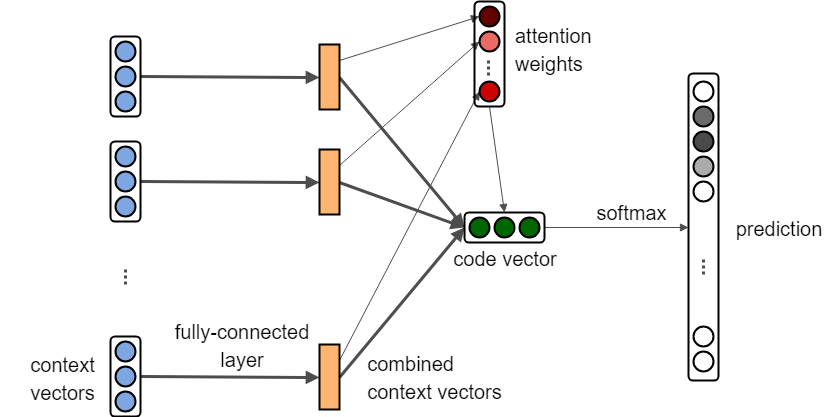
\includegraphics[scale=0.35]{images/modellocode2vec.png}
    \caption{Struttura del modello Code2Vec}
    \label{fig:struttura_modello_code2vec}
\end{figure}